\chapter{Implementacja}
\label{cha:implementacja}

W tym rozdziale opisana jest realizacja praktyczna projektu. Najpierw omówione zostaną wymagania stawiane całej aplikacji i omówione zostaną podstawowe
założenia związane z jej implementacją. Nastepnie przybliżone zostaną jej poszczególne komponenty.

\section{Wymogi i założenia}
\label{sec:wymogi}

\subsection{Budowa}
\label{subs:budowaAplikacji}

Podstawowym celem projektu jest implementacja oprogramowania pobierającego z podzbioru stron opublikowanych w Internecie dokumenty i przedstawiającego
je w postaci omówionych w Rozdziale \ref{cha:budowaGrafu} asocjacyjnych grafów AGDS. Jest to zadanie wieloetapowe, wymagające następujących komponentów:
\begin{enumerate}
\item Robota dostarczającego dane z sieci. Komponent musi mieć możliwość asynchronicznego pobierania stron WWW, udostępniać API do estrakcji adresów URL z ostatnio
ściągniętych stron spełniających podane warunki oraz implementować \emph{Robots Exclusion Protocol}.
\item Komponentu współpracującego z wyżej opisanym modułem, zapweniającego interfejs umożliwiający zapisywanie danych do zewnętrznej bazy. Umożliwiającego
zapisaywanie kolejnych wersji stron WWW, opisanych \emph{timestampem}.
\item Modułu przetwarzającego wybrane strony WWW przechowywane w zewnętrznej bazie. Powinien on być dawać możliwość parsowania strony HTML i operowania na drzewie DOM.
Powinien mieć możliwość zapisu informacji w formacie JSON, przy zachowaniu budowy umożliwiającej proste rozszerzanie funkcjonalności poprzez dodawanie odpowiednich klas do projektu.
\item Prostego klienta kolejki RabbitMQ, wykonującego RPC z przetworzonymi wcześniej danymi, jako argumentem.
\item Serwera odbierającego wywołania przez kolejkę RabbiMQ, rozpoczynającego konwersję danych do formatu AGDS i zwracającego wynik na kolejkę.
\item Modułu przetwarzającego dane odebrane przez serwer, dzielącego wysyłane strony na sekwencje uczące, umożlwiającego w razie potrzeby proste rozszerzenie funkcjonalności.
\item Silnika asocjacyjnego współpracującego z warstwą zapewniajacą persystencję. Jego jedynym zadaniem jest budowa grafu AGDS zgodnie z założeniami opisanymi w Rozdziale
\ref{cha:budowaGrafu}.
\item Warstwy pośredniczącej pomiędzy aplikacją, a bazami danych. Powinna ona zapisywać logiczną strukutrę grafu w bazie grafowej, a dodatkowe informacje, takie jak
atrybuty poszczególnych węzłów(np. częstość występowania), czy krawędzi(np. waga) przechowywać wlekkiej bazie klucz - wartość. Ważne jest ukreywanie szczegółów implementacyjnych,
zwłaszcza wynikających z używania wielu rodzajów baz danych.
\end{enumerate}

Zanim struktura aplikacji zostanie omówiona w większym detalu, należy opisać platformę, na której powstawała. W związku, z faktem, iż implementacja jest pewnego rodzaju eskperymentem, 
od którego nie wyamga się produkcyjnej sprawności, zaimplementowano ją w języku programowania Ruby. Pozwala on na szybką implementację nowych funkcjonalności, jest w pełni obiektowym i
bardzo elastycznym językiem programowania. Jednak związku z tym, iż Ruby jest językiem interpretowanym i posiada dynamiczne typowanie, zaawansowane możliwości metaprogramowania i 
zapewnia rozbudowane mechanizmy refleksji jego wydajność nie jest duża.
W związku z charakterystyką wybranej platformy program ma szanse działać poprawnie jedynie dla systemów typu Unix(Linux, OS X). Zstosowane zostały dwie wersje interepreterów Ruby'ego:
elementy 1. - 4. wymagają interpretera MRI, wersji conajmniej 2.0.0. Jest to pierwsza implementacja tego języka, napisana w C, większość najważniejszych gemów(bibliotek) jest dostępna 
przede wszystkim dla tej dystrybucji. Natomiast moduły 5. - 8. wymagają użycia alternatywnej implementacji na JVM, o nazwie JRuby. Jest to wymaganie używanej bazy grafowej i jest głównym 
powodem użycia kolejki RabbitMQ do komunikacji między dwoma głównymi częściami aplikacji.

Aplikacja używa 3 baz danych: PostgreSQLa(\url{http://www.postgresql.org/}) do przechowywania ściągniętych stron, Neo4j(\url{http://www.neo4j.org/}) jako bazy grafowej i Redisa(\url{http://redis.io/})
 jako lekkiej bazy klucz - wartość. Wszystkie posiadają biblioteki umożliwiające interakcje z nimi na poziomie obiektów języka, co znacznie ułatwia projektowanie aplikacji. Również każda
 z technologii używanych w projekcie jest technologią \emph{Open Source}.
 
 Każdy komponent posiada testy jednostkowe.

\begin{figure}[!h]
    \centering
    \label{graph:aplikacja}
    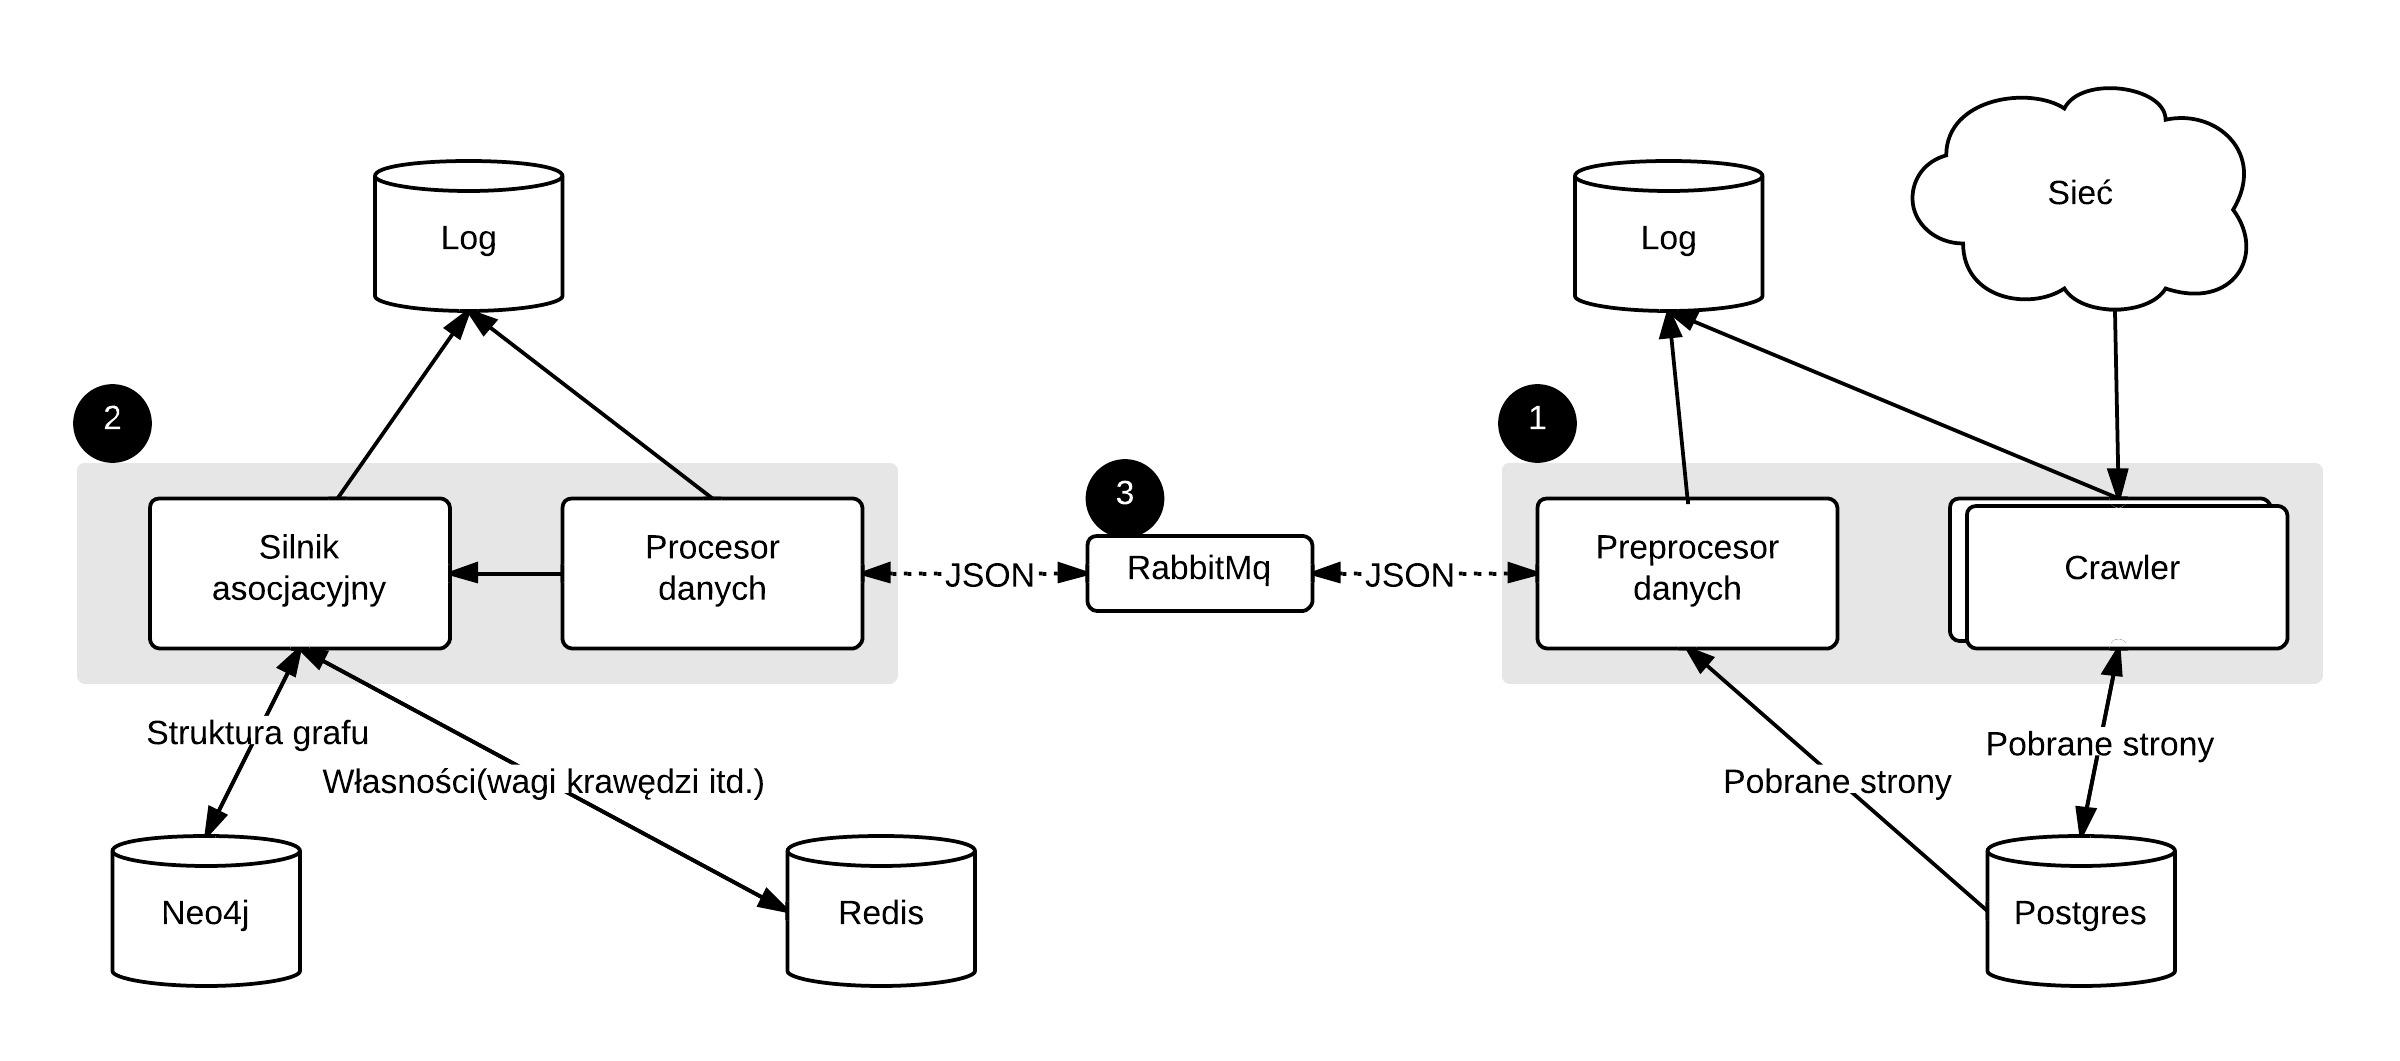
\includegraphics[scale=0.2]{aplikacja}
    \caption{Schemat architektury aplikacji. 1. - część napisana w MRI, 2. - część napisana w JRubym 3. - kolejka}
\end{figure}

\subsection{Wejście/wyjście}
\label{subsec:weWy}

Aplikacja nie posiada interfejsu graficznego. Poszczególne komponenty są wzbudzane z poziomu \emph{shella}, konfiguracja odbywa się poprzez edycję wydzielonych plików konfiguracyjnych, 
opcje podawane przy wykonywaniu skryptów lub zmienne środowiskowe. Celem tej części projektu nie jest serwowanie użytkownikowi informacji, a przedstawianie danych w pewny określonym
formacie, stąd takie ograniczone spektrum możliwości interakcji z aplikacją. Konkretne skrypty uruchamiające aplikacje, opcje ich wywoływania i struktura plików konfiguracyjnych opisana 
jest w dalszej części pracy.

\subsection{Wymagania instalacyjne}
\label{subs:wymaganiaInst}

Aplikacja byla rozwijana i testowana pod systemami typu Unix. Do instalacji i uruchomienia potrzebne są:
\begin{itemize}
\item system kontroli wersji Git (\url{http://git-scm.com/}),
\item Ruby zainstalowany za pomocą systemu kotroli wersji(preferowany rbenv - \url{http://rbenv.org/}),
\item Bundler (\url{http://bundler.io/}) i RubyGems (\url{http://rubygems.org/}),
\item serwer PostgreSQL,
\item baza grafowa Neo4j,
\item serwer Redis.
\end{itemize}

Instrukcje instalacji, konfiguracji i uruchamiania poszczególnych komponentów znajdują się w dalszych częściach pracy.

\section{Opis komponentów 1. - 4.}

Na rysunku \ref{graph:mri} przedstawiony jest detaliczny schemat pierwszych czterech komponentów głównej aplikacji. W istocie tworzą one autonomiczną subaplikację, powiązaną z resztą
komponentów jedynie poprzez kolejkę RabbitMQ. 

\begin{figure}[!h]
    \centering
    \label{graph:mri}
    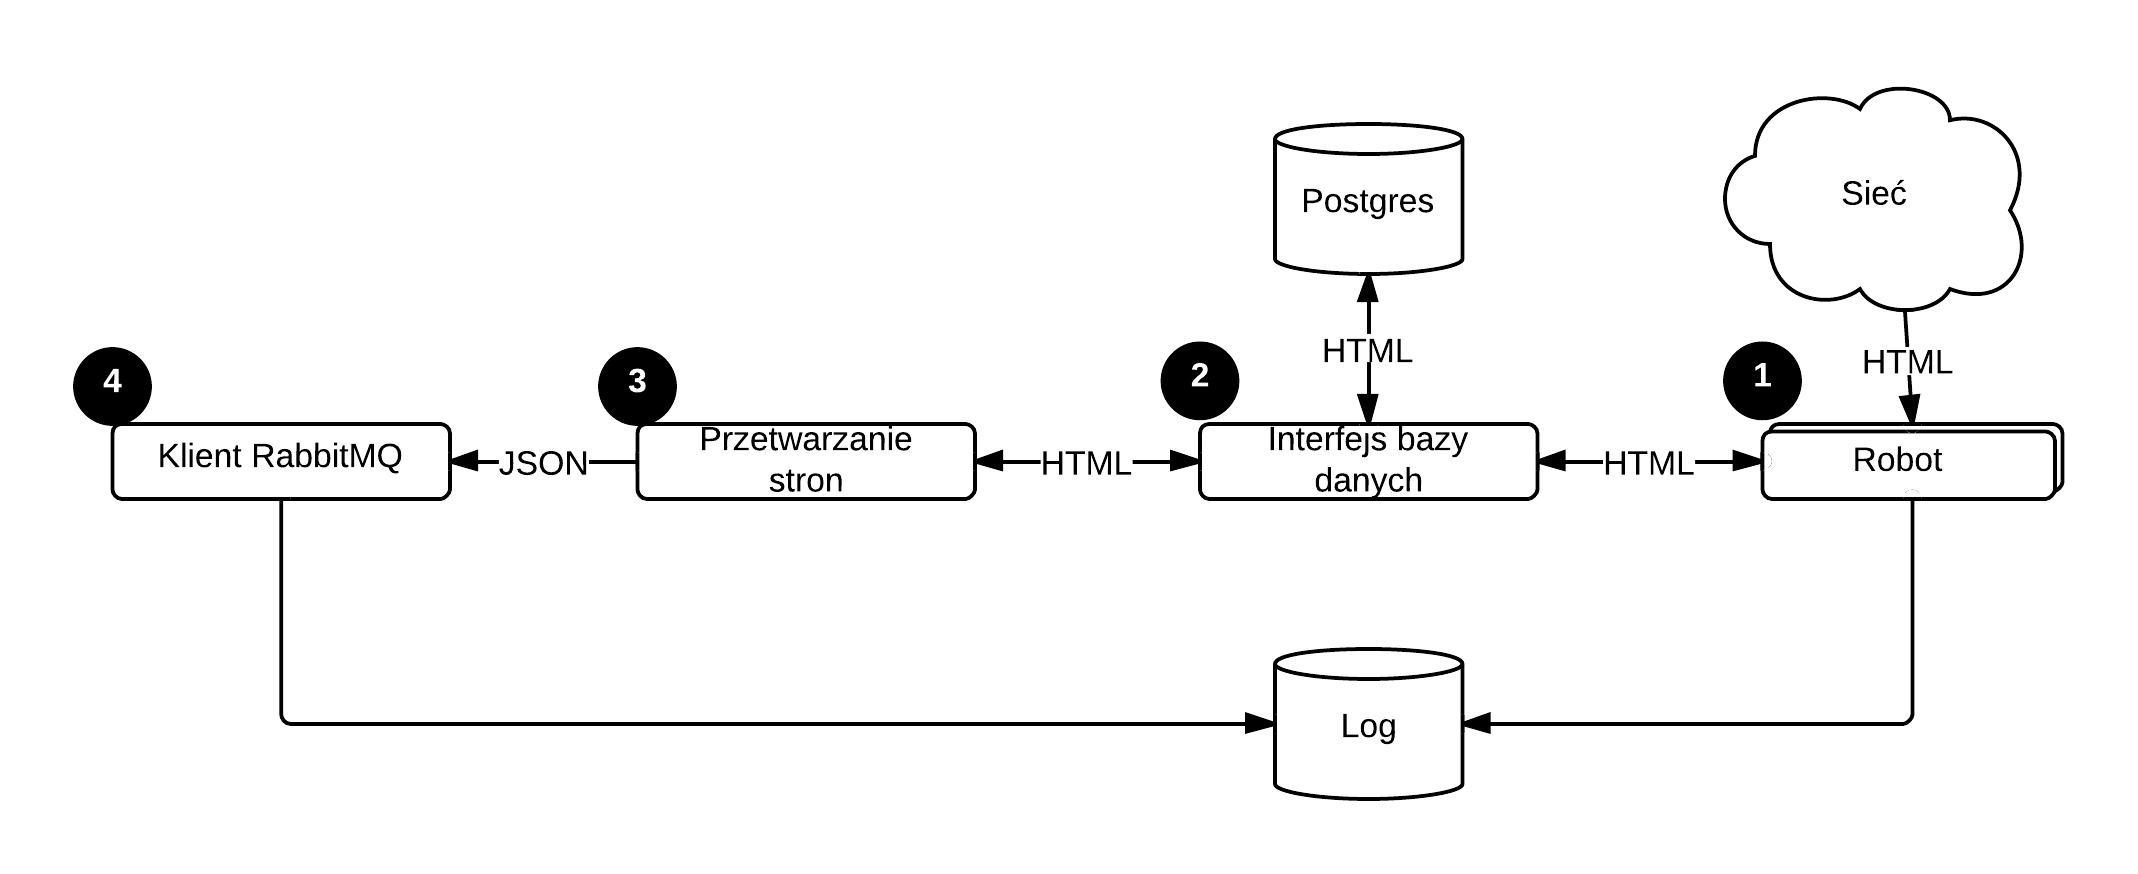
\includegraphics[scale=0.22]{mri}
    \caption{Detaliczny schemat komponentów 1. - 4. Podpisy na strzałkach odnoszą się do formatu, w jakim przedstawiane są strony internetowe na każdym z prezentowanych etapów. }
\end{figure}

\subsection{Konfiguracja}
\label{subs:konfiguracjaMri}

Konfiguracja możliwa jest poprzez dwa pliki znajdujące się w katalogu \texttt{./config}: \texttt{database.yml} i \texttt{config.yml}. Umożliwiają one dostarczenie potrzebnych
informacji pozwalających na połączenie z relacyjną bazą danych, jak i na konfigurację zachowania aplikacji. Poniżej przedstawiony jest listing obu plików 
wraz z wyjaśnieniem dostępnych opcji.

\texttt{database.yml}

\lstset{language=ruby}
\begin{lstlisting}[frame=single]
defaults: &defaults
  adapter: postgresql
  encoding: unicode
  pool: 5
  username: user
  password: pass
  host: localhost

development:
  database: taskmaster_dev
  <<: *defaults
test:
  database: taskmaster_test
  <<: *defaults

\end{lstlisting}

Jest to plik instrumentujący używany w aplikacji ORM - \emph{Active Record}, w celu umożliwienia połączenia z bazą. Konieczne podanie jest typu(\emph{adapter}), 
użytkownika(\emph{user}), hasła(\emph{password}) i lokazlizacji bazy(\emph{host}). Zdefiniowano również specjalne środowisko testowe, dostępne pod luczem \texttt{test}.
Służy ono do definicji bazy powoływanej do egzystencji na czas testów, a następnie bezpowrotnie niszczonej. 

\texttt{config.yml}

\lstset{language=ruby}
\begin{lstlisting}[frame=single]
crawler:
  connections: 20
  fetch_limit: 20
  url_pattern: '\/\/en\.wikipedia\.org\/wiki\/(?!\/|[A-Za-z]+:)'
  starting_page: 'http://en.wikipedia.org/wiki/Main_Page'
  polite: true
  request_gap: 1
queue:
  limit: 50
logger:
  file: 'log/development.log'
  enabled: true

\end{lstlisting}

Plik ten przechowuje informacje konfiguracyjne aplikacji. Kolejno, odpowiadają one za:
\begin{itemize}
\item \texttt{crawler: connections} mówi, ile jednoczesnych asynchronicznych połączeń może wykonywać jeden proces robota.
\item \texttt{crawler: fetch_limit} określa, ile na raz URLi jest wysyłanych do robota w celu ściągnięcia z Internetu. Nie jest t jednoznaczne z parametrem \texttt{connections}, 
w razie wysłania większej ilości adresów URL, niż jest otwieranych połączeń crawler wykona kilka iteracji i zwróci dokumenty odpowiadające wszystkim adresom.
\item \texttt{crawler :starting_page} przechowuje 
\end{itemize}


Łatwo zauważyć, iż dwie pierwsze części tworzą implementację pająka sieciowego, przedstawionego w rozdziale \ref{cha:pozyskiwanieTresci}. Trzeci moduł, 
zaprojektowany jest tak, by umożliwić możliwie najbardziej elastyczny sposób przetwarzania danych, umożliwiający proste dodawnie owych komponentów bez edycji 
istniejącej logiki (zgodnie z regułami programowania obiektowego, szczególnie tzw. \emph{Open - Closed Principle} \cite{ooPrinc}).

Interakcja z modułem opiera się na wywoływaniu w  \emph{shellu} odpowiednich skryptów. 
